\documentclass{sig-alternate}
\usepackage{amsfonts,xspace}
\usepackage{url}
\usepackage{epsfig}
\usepackage{graphicx}
\usepackage{subfigure}
\usepackage{ifpdf}
\usepackage[usenames,dvipsnames]{color}
\newcommand{\tbd}[1]{}
\newcommand{\ie}{{\it i.e.}}
\newcommand{\eg}{{\it e.g.}}
\newcommand{\etc}{{\it etc.}}
\newcommand{\eat}[1]{}
\usepackage[english,plain]{fancyref}
\usepackage{times}
\usepackage{rotating}
\usepackage[labelformat=simple]{subfig}


\newcommand{\mypara}[1]{\medskip\noindent{\bf {#1}:}~}
\newcommand{\chk}{$\checkmark$}
\newcommand{\dsh}{{\bf --}}
\newcommand{\til}{{\bf\large \textasciitilde}}
%\newcommand{\tbd}[1]{[{\color{red}{\bf{TBD: #1}}}]}
\newcommand{\etal}{\emph{et~al.}}
\newcommand{\meddle}{{Meddle}\xspace}
\newcommand{\dsum}{\displaystyle\sum}
\newcounter{packednmbr}

\newenvironment{packedenumerate}{\begin{list}{\thepackednmbr.}{\usecounter{packednmbr}\setlength{\itemsep}{0.2pt}\addtolength{\labelwidth}{-4pt}\setlength{\leftmargin}{\labelwidth}\setlength{\listparindent}{\parindent}\setlength{\parsep}{1pt}\setlength{\topsep}{0pt}}}{\end{list}}
\newenvironment{packeditemize}{\begin{list}{$\bullet$}{\setlength{\itemsep}{0.2pt}\addtolength{\labelwidth}{-4pt}\setlength{\leftmargin}{\labelwidth}\setlength{\listparindent}{\parindent}\setlength{\parsep}{1pt}\setlength{\topsep}{0pt}}}{\end{list}}
\newenvironment{packedtrivlist}{\begin{list}{\setlength{\itemsep}{0.2pt}\addtolength{\labelwidth}{-4pt}\setlength{\leftmargin}{\labelwidth}\setlength{\listparindent}{\parindent}\setlength{\parsep}{1pt}\setlength{\topsep}{0pt}}}{\end{list}}

\renewcommand{\fref}{\Fref}
\renewcommand\thesubfigure{~(\alph{subfigure})}

\title{\meddle: Middleboxes for Increased Transparency and Control of
  Mobile Traffic\vspace{-0.2in}}

% middlebox transparency control mobile traffic 
\numberofauthors{6}
\author{
\alignauthor
Ashwin Rao\\
\affaddr{INRIA}
\alignauthor        
David Choffnes\\
\affaddr{University of Washington}
\alignauthor
Justine Sherry\\
\affaddr{UC Berkeley}
\and
\alignauthor
Arnaud Legaut\\
\affaddr{INRIA}
\alignauthor 
Arvind Krishnamurthy\\
\affaddr{University of Washington}
\alignauthor
Walid Dabbous\\
\affaddr{INRIA}
}
\begin{document}	
%http://www.sheridanprinting.com/typedept/conextstudent.htm
\conferenceinfo{CoNEXT Student'12,} {December 10, 2012, Nice, France.}
\CopyrightYear{2012}
\crdata{978-1-4503-1779-5/12/12}
\clubpenalty=10000
\widowpenalty = 10000

\maketitle

\begin{abstract}
In this poster we present \meddle, a framework aimed at enhancing
the transparency in mobile networks and providing a platform that lets
users reclaim control over their mobile traffic. We use our working
prototype to show that \meddle, which builds upon VPNs and
middleboxes, is feasible to implement, and is capable of providing
sufficient incentives to conduct large scale experiments and user
based measurement studies.
\end{abstract}

\section{Introduction}

In the mobile environment, users are forced to interact with a single
operating system tied to their device, generally use closed-source
apps that routinely violate user privacy~\cite{hornyack:appfence}, and
subscribe to network providers that can (and do) transparently modify,
block or otherwise interfere with network
traffic~\cite{wang:middleboxes}.  

Researchers face a similar set of challenges for characterizing an
experiment for mobile systems. To characterize mobile traffic and
design new protocols and services that are better tailored to the
mobile environment, we would like a framework that allows us to
intercept and potentially modify traffic generated by mobile devices
as they move with users, regardless of the device, OS, wireless
technology, or carrier. However, implementing this functionality is
difficult on mobile devices because it requires warranty-voiding
techniques such as jail breaking to access and manipulate traffic at
the network layer~\cite{enck:taintdroid}. Even when using such an
approach, carriers may manipulate traffic once it leaves the mobile
device~\cite{wang:middleboxes}, thus rendering some research
impractical. Furthermore, researchers generally have no ability to 
deploy solutions and services such as prefetching and security
filters, that should be implemented in the network.

In this poster, we present \meddle, a framework that combines
VPNs with middleboxes to align the interests of users and
researchers. \meddle relies on VPN tunnels to route mobile traffic
through it regardless of the device, OS, wireless technology, and
carrier. \meddle can thus provide a continuous and
comprehensive view of how mobile devices interact with the
Internet. Once packets arrive at a \meddle server, we use a variety of
middlebox approaches to transform traffic to and from mobile devices.

We believe \meddle offers a strong research platform for both,
measuring and characterizing mobile traffic, and designing new
in-network features to improve the mobile experience. For example, the
comprehensive view of mobile traffic regardless of the wireless
technology can help us determine how different operating systems and
apps offload their traffic from 3G or 4G networks to Wi-Fi. To
improve the user experience, we currently implement packet filters
to block ads; such packet filters currently require jail-breaking the
mobile device. Furthermore, Meddle provides an ideal vantage point for
separating mobile-network performance from server-side performance,
thus improving bottleneck identification for mobile
applications. \meddle also enables researchers to investigate what-if
scenarios for the impact of new middleboxes as if they were deployed
in carrier networks. For example, \meddle can be used to deploy and
test anonymization systems such as Privad~\cite{guha:privad}. 

\section{\meddle Architecture}

\begin{figure}
  \centering
  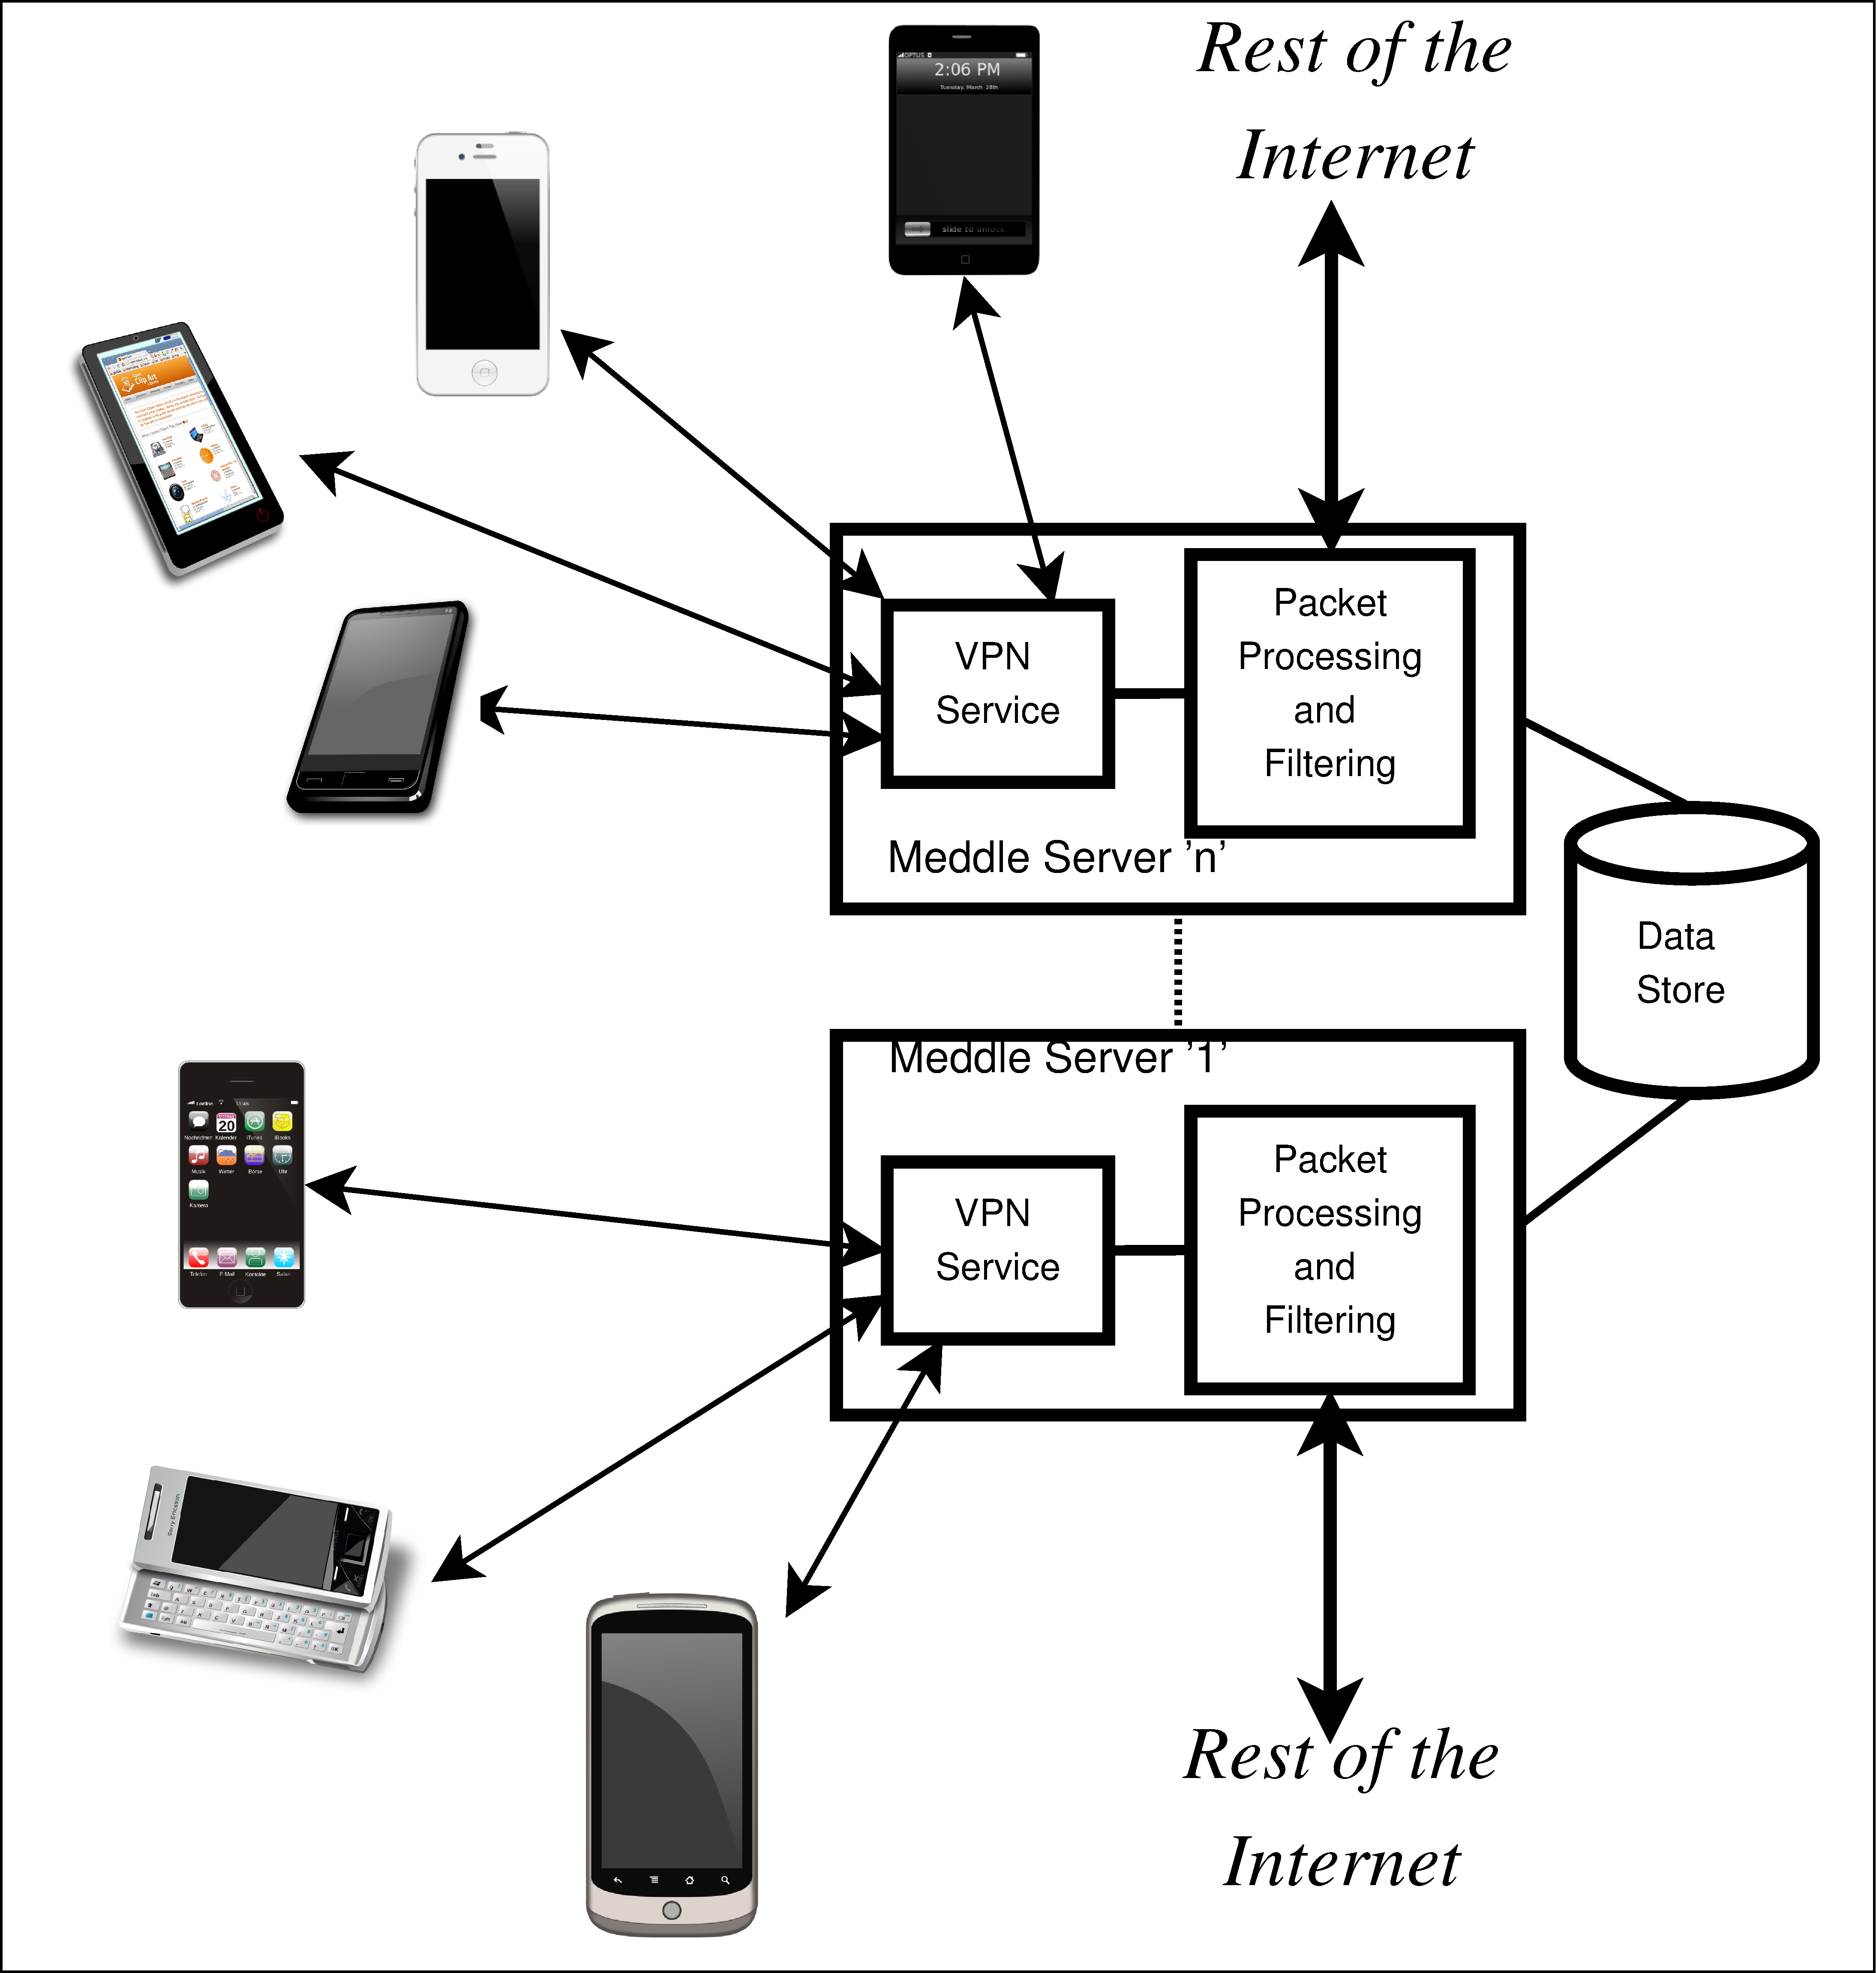
\includegraphics[width=0.65\columnwidth]{figures/meddle-servers.eps}
  \caption{System schematic. \emph{Clients connect to a nearby \meddle
      server. Client data is stored in a shared data store.}} 
  \label{fig:MeddleDeployment}
\vspace{-0.08in}
\end{figure}

\meddle uses VPNs as a portable mechanism to tunnel the data traffic
from mobile devices to a machine whose functionality can by controlled
by the user and used by researchers for the purpose of analysis and
interposition. VPNs also reduce the entry barrier to deploy \meddle
because Android, BlackBerry, and iOS, that represent more than 86\% of
the mobile device market~\cite{gartner-phone-share}, have native VPN
support. As shown in \fref{fig:MeddleDeployment}, when a mobile device
connects to the Internet, we tunnel its traffic via a nearby \meddle
server in a similar way to how the Akamai CDN uses DNS to redirect Web
clients to nearby content caches~\cite{akamai:cdn}. Currently, on each
\meddle server we (a) implement custom services for users such as
packet filtering, caching, and intrusion detection, and (b) monitor the
network traffic characteristics. \meddle thus takes two well-known
technologies -- VPNs and middleboxes -- and combines them in
unintended ways for the mobile environment

\meddle requires minimal inputs from end users. For iOS devices, we
use the iPhone Configuration Utility to generate a user specific
profile that creates and manages the VPN tunnel. Once the user installs
this profile, all the data traffic from the iOS  device is tunneled
through the \meddle servers. For Android devices, we use a modified
Strongswan app because of some bugs related to reconnection in the
native VPN  implementation~\cite{OnDemandAndroid}. A user needs to
enter the credentials for the VPN tunnels only once, during the
installation of the Strongswan app. To manage VPN tunnels on each
\meddle server, we use StrongSwan~\cite{strongswan}, an open-source
VPN implementation that uses native IPsec functionality.   

\section{Case Studies}

We believe that the research enabled by \meddle shall form a positive
feedback loop in which new, proven research artifacts become
additional incentives for user adoption, thus enabling further
research. We currently have a prototype of \meddle which is running
from August 27, 2012 and serving 9 different mobile devices which
includes an Android phone, an iPhone, an iPad, and an iPod
Touch. Users that are part of an IRB approved study to characterize
mobile traffic are currently using these devices. 

\textbf{\meddle example.} We have implemented a DNS based filter to
block ads, analytics, and mediation sites. We believe that such a filter is
an important incentive for a user based study because
Vallina-rodriguez~\etal~\cite{Vallina-rodriguez:2012:AdCache} observe
that ads account for 5\% of daily traffic from more than 50\% of
Android users in a large European ISP. We use the recent research on
mobile ads~\cite{hornyack:appfence, Leontiadis:2012:AdsMobile} and a
publicly available list of domains~\cite{YoyoAds} to filter
domains specific to mobile networks. We observed a 0.05\% to 0.8\%
reduction in total traffic at each mobile device due to our ad
blocking engine.  

\begin{table}
\centering
\begin{small}
\begin{tabular}{|l|l|l|l|l|}
\hline
{\bf User} & {\bf Home} & {\bf Work} & {\bf Mobile} & {\bf Volume}\\
    & {\bf (Wi-Fi)} & {\bf (Wi-Fi)} & {\bf (3G)} & {\bf (GB)}\\
\hline
User 1 & 84.4\% & 11.9\% & 3.7\%  & 1.23 GB\\
\hline
User 2 & 95.1\% & 4.2\% & 0.7\%  & 1.42 GB\\
\hline
\end{tabular}
\end{small}
\caption{Traffic share and volume from two iPhones when using Wi-fi at
  home, Wi-Fi at work, or a 3G connection. \emph{A significant
    fraction of traffic from our users come from Wi-fi networks.}}
\label{tab:Usage}
\vspace{-0.1in}
\end{table}

\textbf{Measuring Traffic Offload.} In \fref{tab:Usage}, we summarize
the traffic volume observed from two iPhone users, one in the US and
the other in France, for 20 days from August 27, 2012. The two users
generated a traffic of 2.65 GB that passed through our \meddle
server. In \fref{tab:Usage}, we observe that the 3G traffic contributes
to a very small fraction of the total traffic from the
two iPhones. We do not present results from Android devices because we
began our study using the native VPN implementation for Android that has
reconnection issues~\cite{OnDemandAndroid}; we recently resolved these
issues by modifying the Strongswan app, an alternative to the native
VPN implementation.  

\textbf{Overhead.} We observe low overheads in terms of power
consumption, data quota, and network latency, when tunnelling data
traffic via a VPN. We observed a 10\% increase in power consumption
when streaming an HD video from YouTube to an Android device and an
iPhone via one of our \meddle servers. We measured the overhead of the
tunnel in terms of data overhead from IPsec headers and keepalive
messages, finding that it ranges from 8--12\% for an Android phone and
an iPhone. Our test traffic included Web searches, interaction on
social networks, map searches, playing a game, online shopping,
downloading popular apps, emailing and reading the news. To address
the increase in network latency we envision a DONAR-style deployment
where users are dynamically redirected to a \meddle based on network
conditions and server load~\cite{wendell:donar}. We observe that
PlanetLab nodes have a latency between 3\,ms and 13\,ms, with a median
of 5\,ms from the mobile-network egress points. We used the data
collected from 10 mobile phones located throughout the US for this
measurement study. Thus, when compared to RTTs of 10s or 100s of
milliseconds that exist in mobile networks, the additional latencies
from traversing a \meddle server is expected to be relatively small or
even negligible.  

\section{Future Work}

% \begin{figure}
%  \centering
%  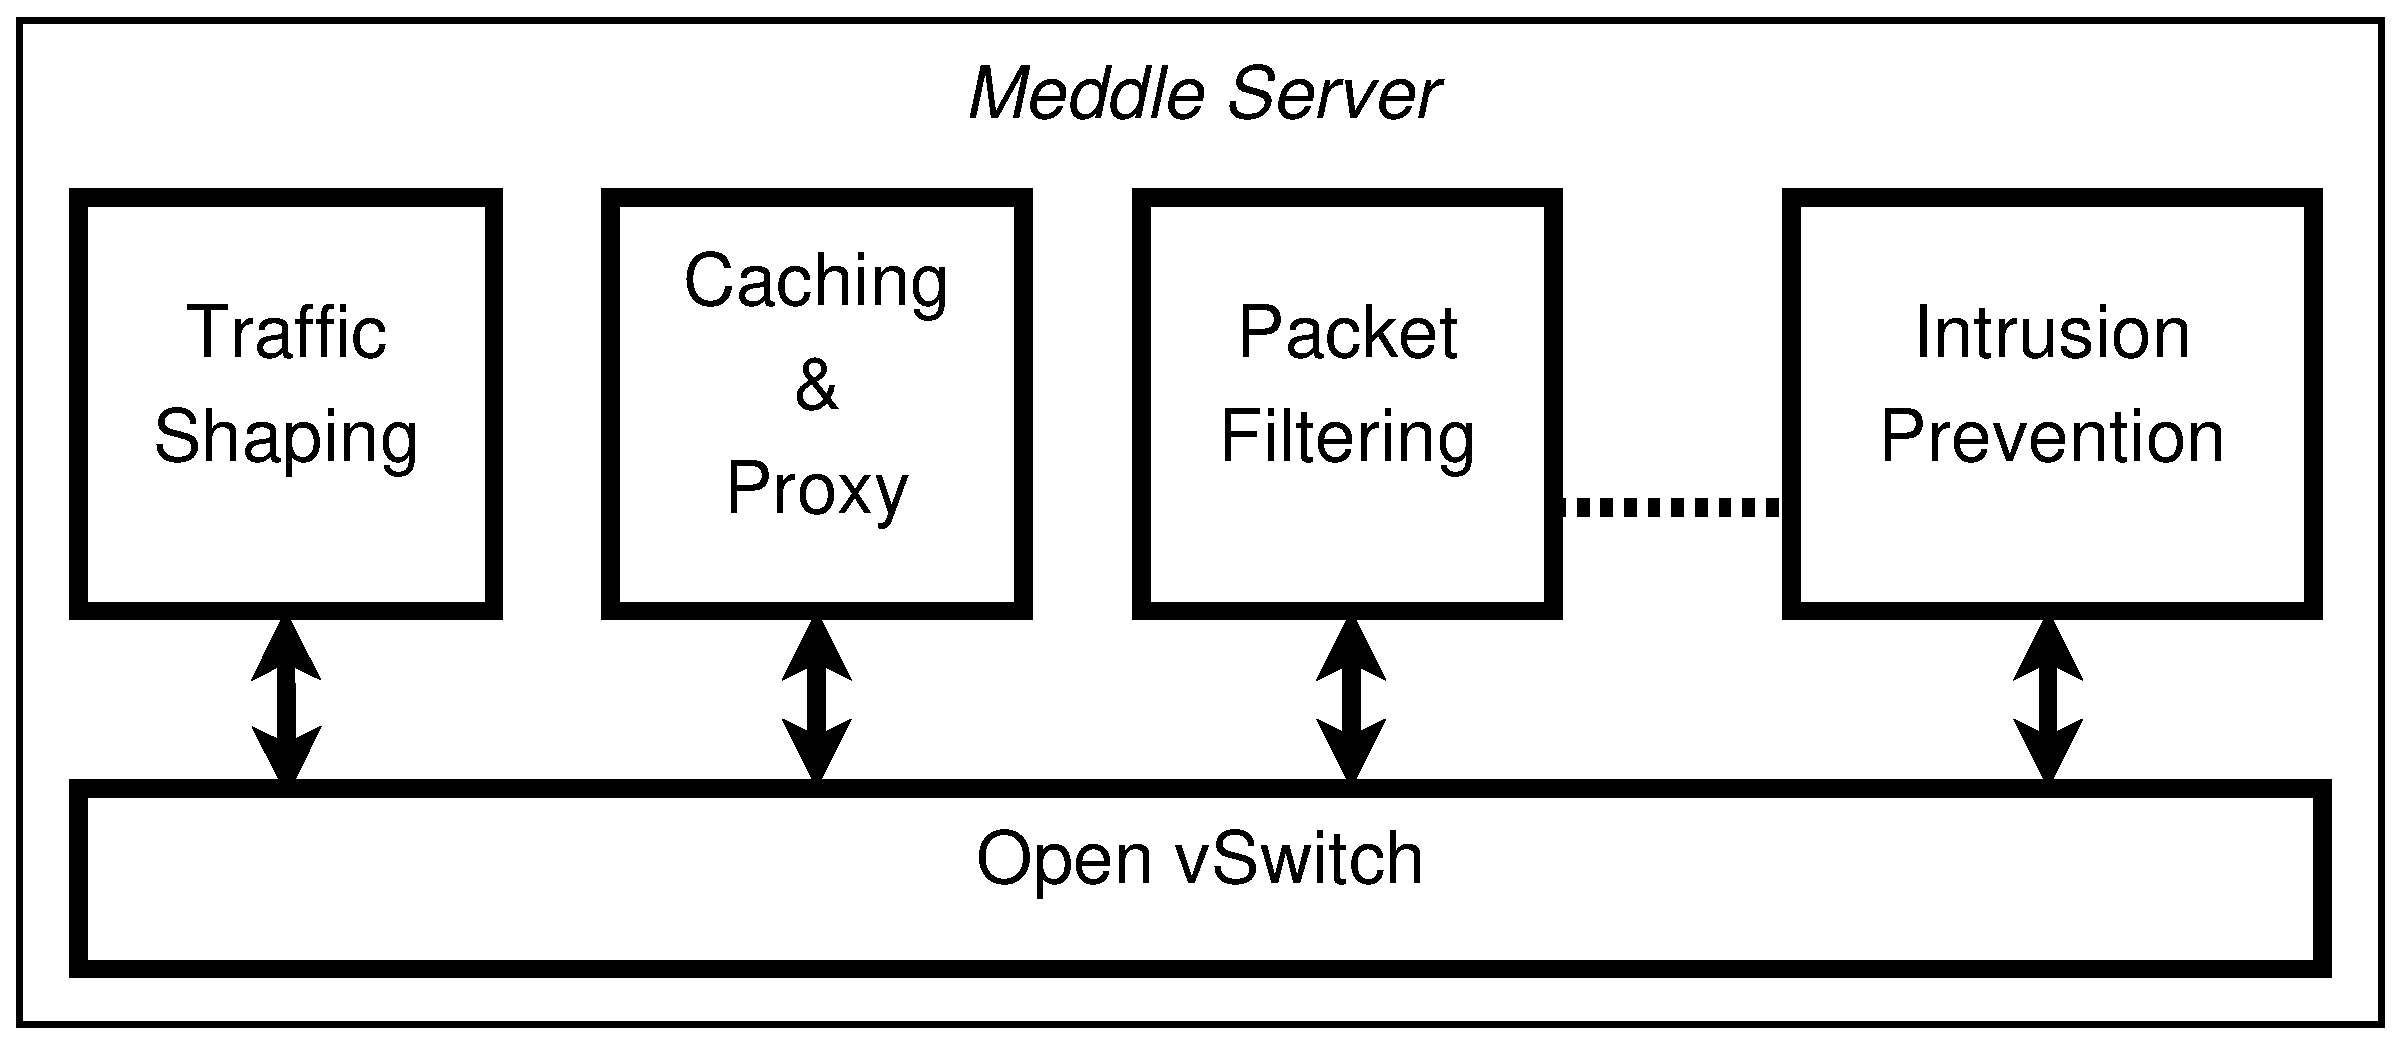
\includegraphics[width=0.65\columnwidth]{figures/OpenSwitch.eps}
%  \caption{Virtual machines on each \meddle server. \emph{Each virtual
%      machine addresses a specific problem.}}
%  \label{fig:OpenSwitch}
% \vspace{-0.09in}
% \end{figure}

We are currently recruiting users for an IRB approved study on the
network usage profiles of mobile phone users. To enhance the
transparency of mobile networks, we plan to allow users see how
the installed apps use the network and with whom these apps share (or
leak) information; a system similar to Mozilla
Collusion~\cite{collusion}. We plan on using Open
vSwitch~\cite{Openvswitch} on each \meddle server to route packets
through virtual machines depending on the source of the traffic and
the protocols used to create the
packets~\cite{Sekar:2012:ConsolidatedMBox}. This architecture enables
us to test algorithms for content coalescing, caching, prefetching,
and offloading the work of processing the DOM to speed up page load
times~\cite{opera-mini, silk, google-spdy}. 

%  Furthermore, we envision
% that most of the interesting opportunities for mobile offloading will
% come at the intersection of severe constraints for mobile devices
% (power, data volume quota, and latencies) and the applications that
% extensively exercise those constraints. For instance, distributed hash
% tables (DHTs) are an example of a distributed service that has become
% critical for a variety of applications from P2P communication to
% content caching and anonymous networking. Using a split-application
% model, mobile device need only send a request for a key to the
% server-side and the server can perform all the network operations
% required to locate the value without consuming mobile network
% bandwidth. 

\begin{small}
\bibliographystyle{abbrv}
\bibliography{related_work}
\end{small}
\end{document}
